\section{Cross-Validation}
\subsection{k-fold Cross-Validation}
Without Crossvalidation: Train 1 Model with 80\% of the Data and Test with 20\%.\\
With \textbf{k-fold:}\\
Repeat the split-train-test procedure for k times.\\
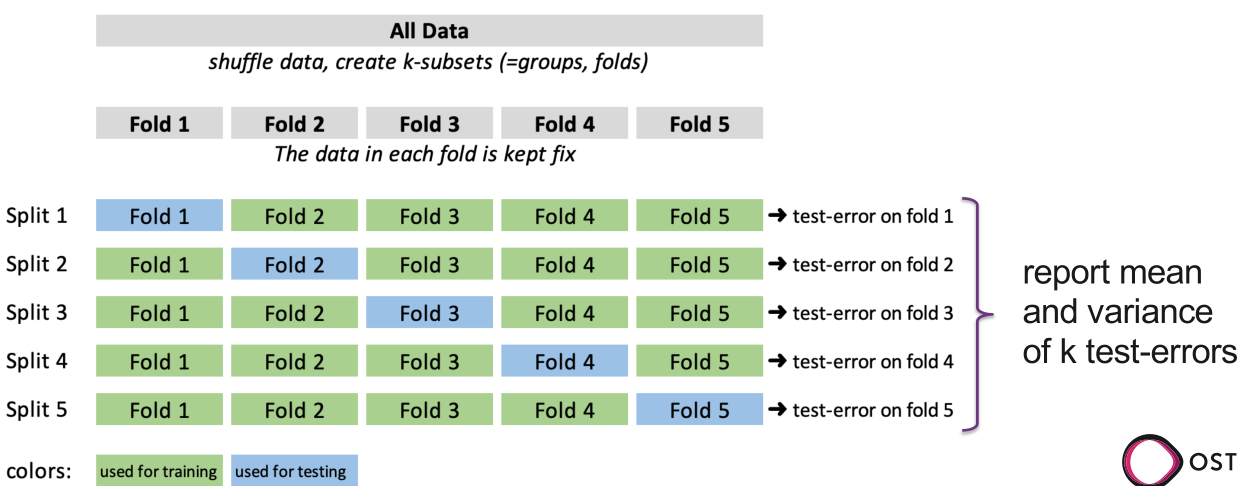
\includegraphics[width=\linewidth]{k-fold.png}\\
E.g.: Split into k = 5 folds.
A Datapoint is fixed in the fold, so no shuffling afterwards.
Then test k times, each time with a different fold as test data. 
Every split is used as test data once.
\subsubsection{Comments}
Typical values are 5, 10 or N.\\
\textbf{k = N} is good for small datasets. 
Every datapoint is in a single fold, and every datapoint is at least once a test set as single datapoint.
Bad for huge datasets, as it has to run N times.\\
\textbf{Preprocessing:} Do not preprocess the whole dataset, but for each split (Calculation mean and variance).

\subsection{k-fold - Use Case 2}
\textbf{model parameter:} Usually weights of the model, like param a and b.\\
\textbf{hyper parameters:} Params for training procedure (regularization parameter $\lambda$)\\
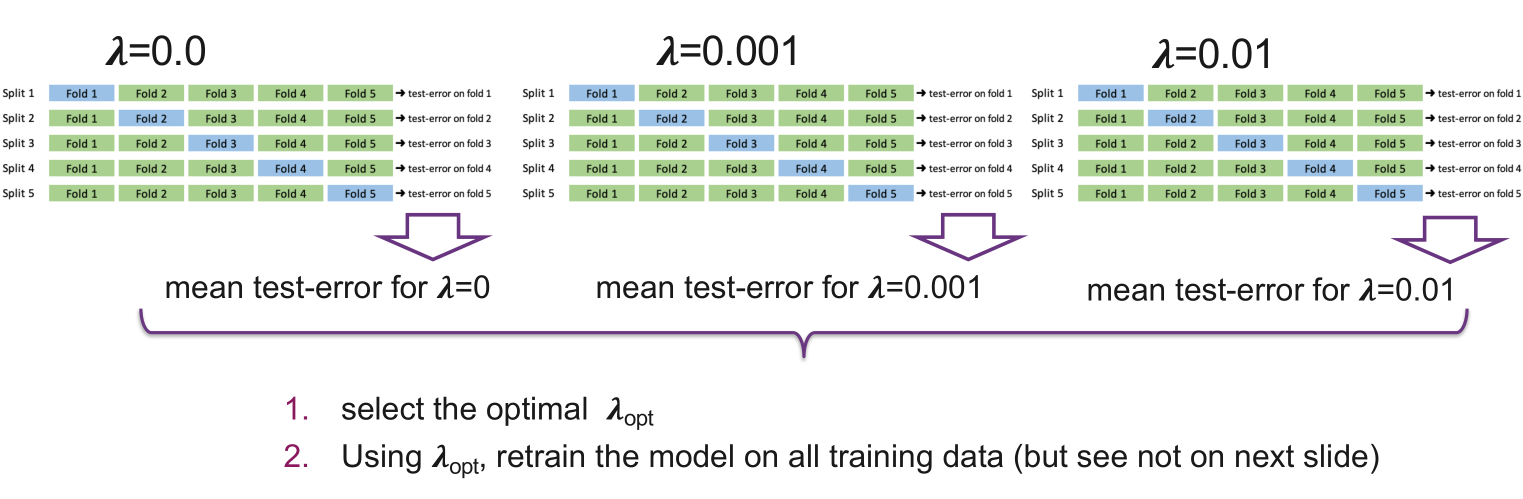
\includegraphics[width=\linewidth]{k-fold-lamda.png}\\
Lambda is often selected on logaritmic basis and very small.

\subsection{scikit-learn: Cross-Validation}
Take a dataset at the beginning, and do not use it \textbf{at all} until the end.
This helps for a final evaluation. 
Do useful for really small datasets, like 10 patients with rare diseases, because you cannot just leave two away.\\
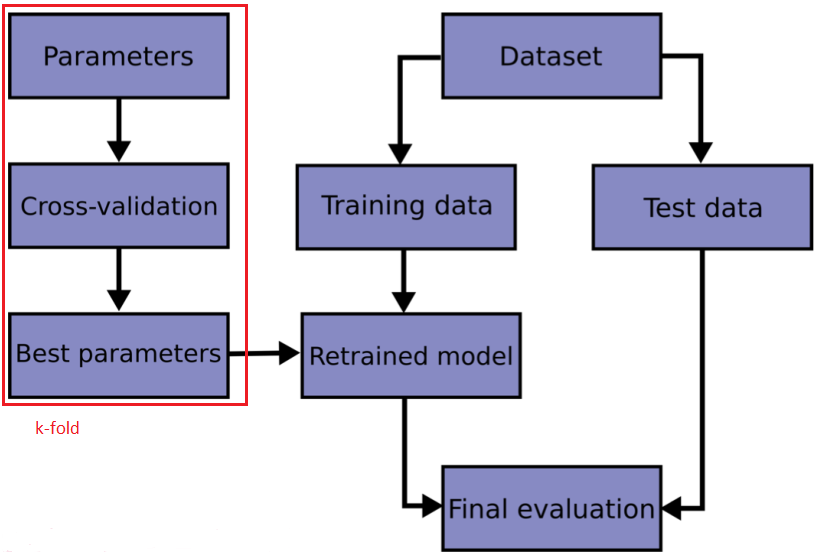
\includegraphics[width=\linewidth]{scikit-cross-validation.png}

\section{ANN (Artificial Neural Networks)}
\subsection{Artifical Neurons}
The artificial neuron receives an input vector multiplied with a weight.\\
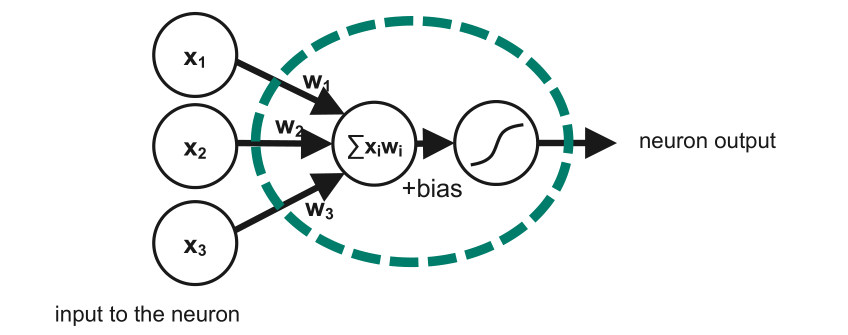
\includegraphics[width=\linewidth]{neuron-io.png}\\
The neuron calculates the sum adds a bias \textbf{b} and passes it thorugh a \textbf{nonlinear} activation function.\\
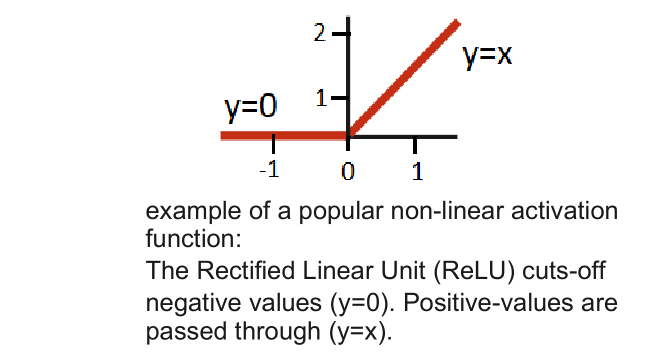
\includegraphics[width=\linewidth]{neuron-activation-function.png}
\textbf{Bias} here is not the same as in the Trade-Off. Here it is the height on the x scale (a*x + \textbf{b}).

\subsection{A simple ANN}
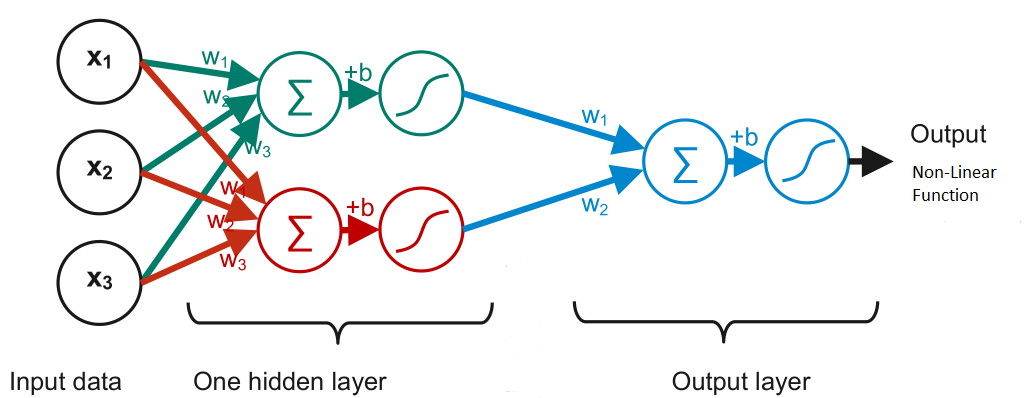
\includegraphics[width=\linewidth]{simple-ann.png}
This ANN has: 2 Layers, 3 Neurons, 11 trainable params.\\
\textbf{Parameters:} The Weights and the Bias of each neuron.

\subsection{A complex ANN}
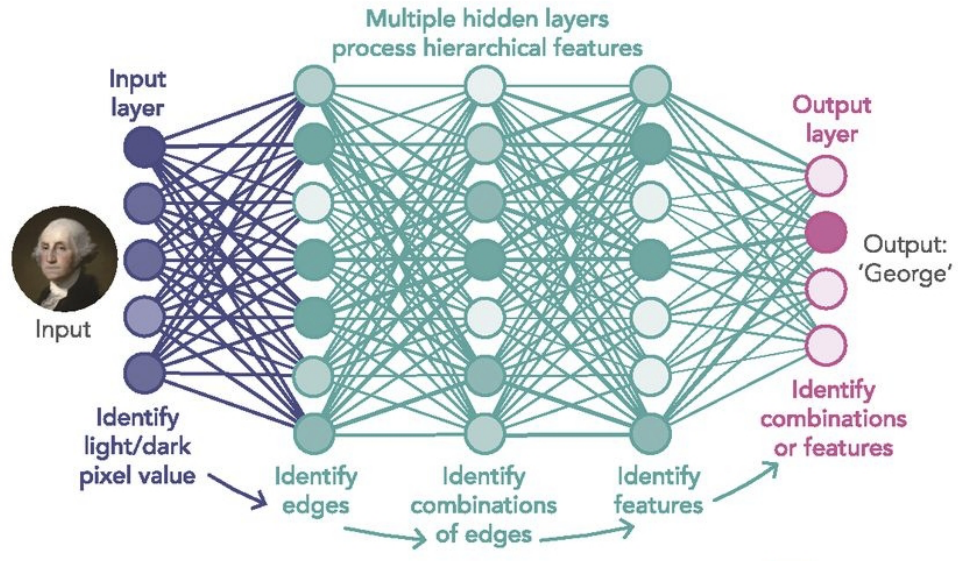
\includegraphics[width=\linewidth]{complex-ann.png}\\
ANN with multiple hidden layers are called \textbf{deep} neural networks.

\subsection{How to train an ANN}
The ANN is initialized with random weights and produces an output.
Then, an optimizer (e.g.: SGD) reduces the cost-function (e.g.: MSE).
Aat every iteration, for every weight and bias, the partial derivative $\frac{\partial}{\partial w}(y - \hat{y})^2$ is calculated.
This is done with the Algo \textbf{Backpropagation}\\
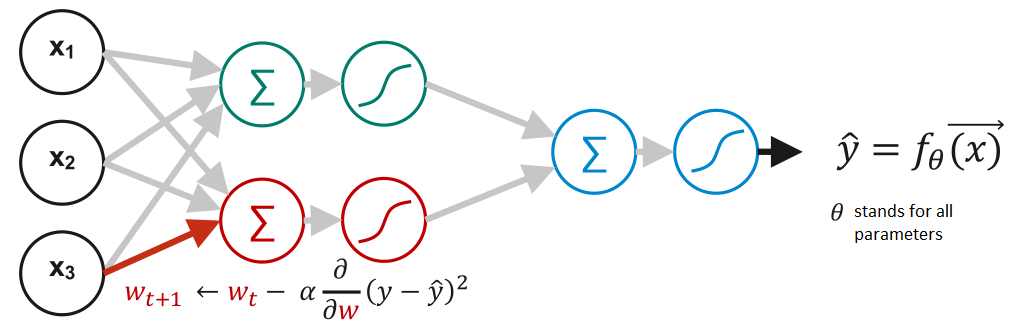
\includegraphics[width=\linewidth]{train-ann.png}
\subsection{ANN in Computer Science}
An ANN is a data-structure calles expression-tree. 
Each node can be evaluated.
Finding the optimal weigths is only possible because of the Backpropagation Algo.\\
Math perspective: Backpropagation is basically the chain rule.\\
CS perspective, Backpropagation is a recursive, Dynamic-Programming algorithm.




